\chapter{Feature Extraction}
\label{ch:Feature Extraction}

\section{Line extraction}
In order to extract the most significant lines:
\begin{enumerate}
    \item Crop the image to the desired portion
    \begin{figure}[H]
    \centering
    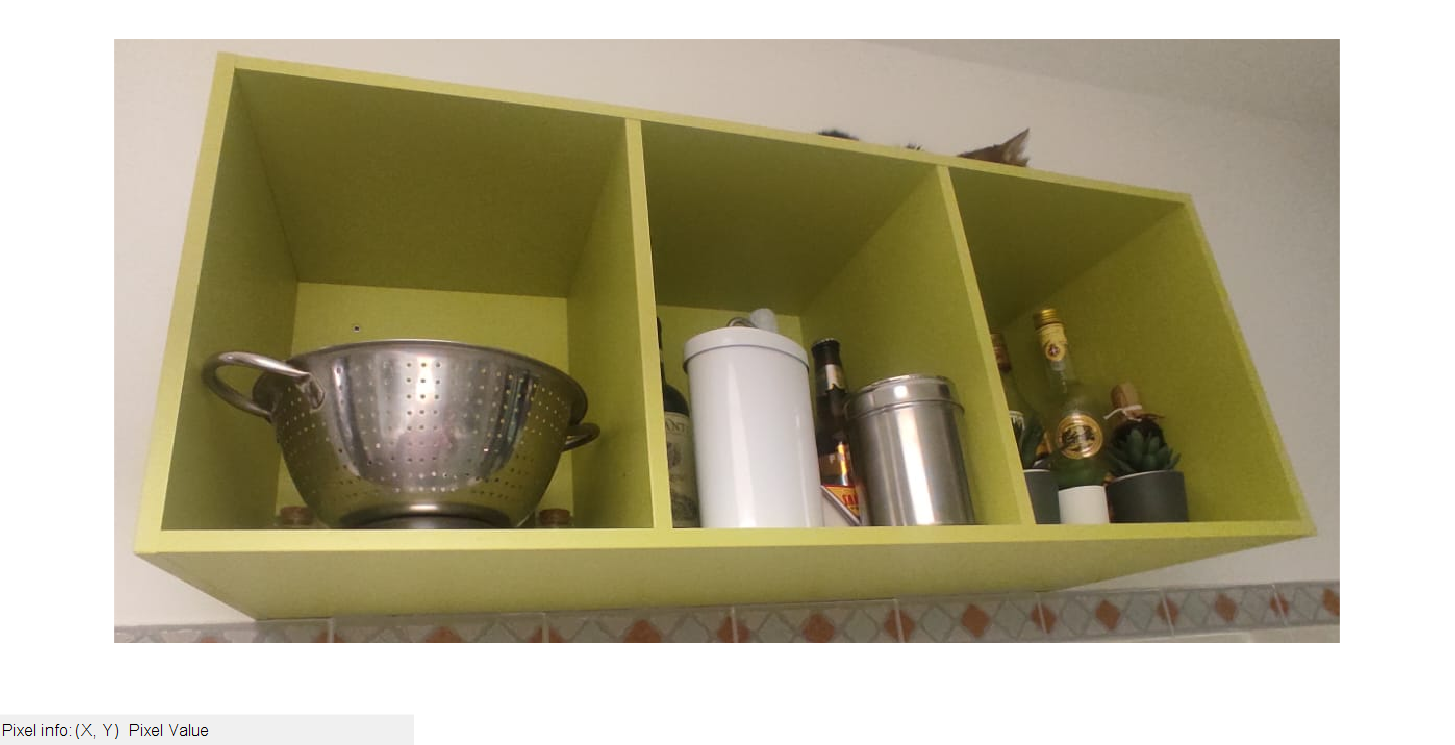
\includegraphics[height=9.5cm, width=\textwidth, keepaspectratio]{Report/Images/Features/Lines/CroppedImage.png}
    \caption{\label{fig:lines:cropped}The image cropped}
    \end{figure}

    \item Convert to HSV color space.

    \item Perform the SVD on the RGB channels plus the Saturation and Value.

    \begin{figure}[H]
    \centering
    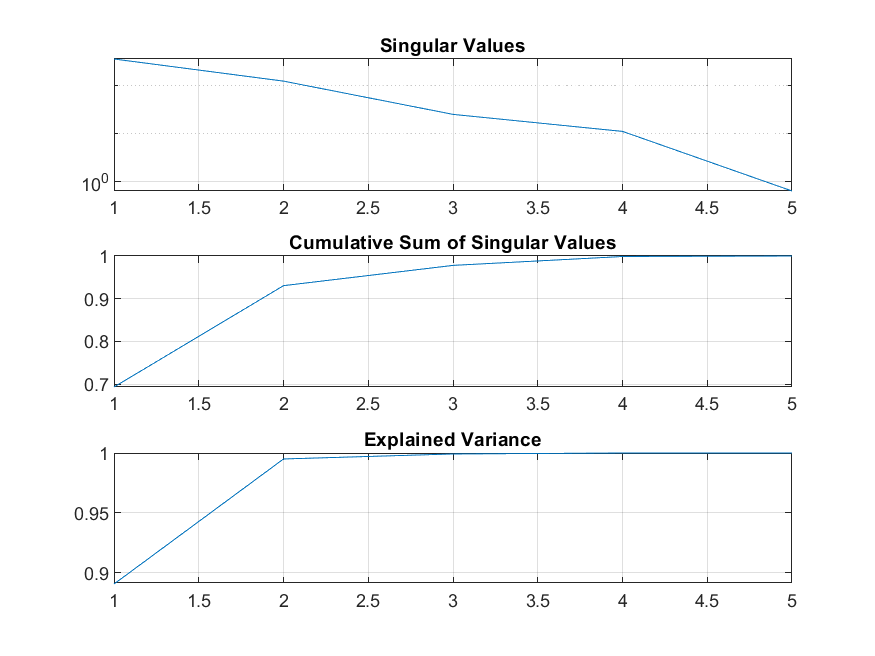
\includegraphics[height=9.5cm, width=\textwidth, keepaspectratio]{Report/Images/Features/Lines/SingularValues.png}
    \caption{\label{fig:lines:sv}The singular values distribution}
    \end{figure}

    \item Compute the Principal Components
    \begin{figure}[H]
    \centering
    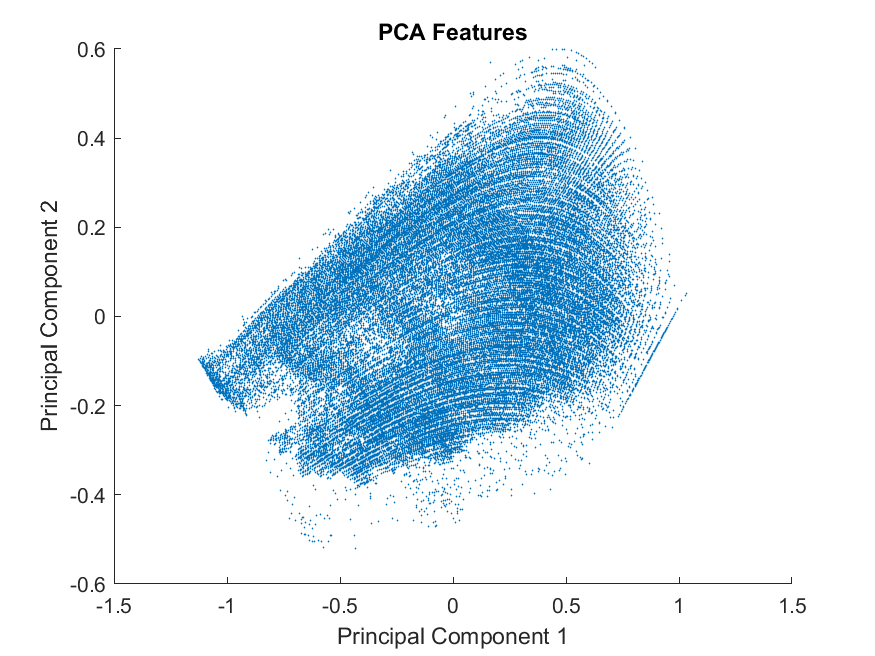
\includegraphics[height=9.5cm, width=\textwidth, keepaspectratio]{Report/Images/Features/Lines/PCAFeatures.png}
    \caption{\label{fig:lines:pc 2d}The first 2 principal components}
    \end{figure}

        \begin{figure}[H]
    \centering
    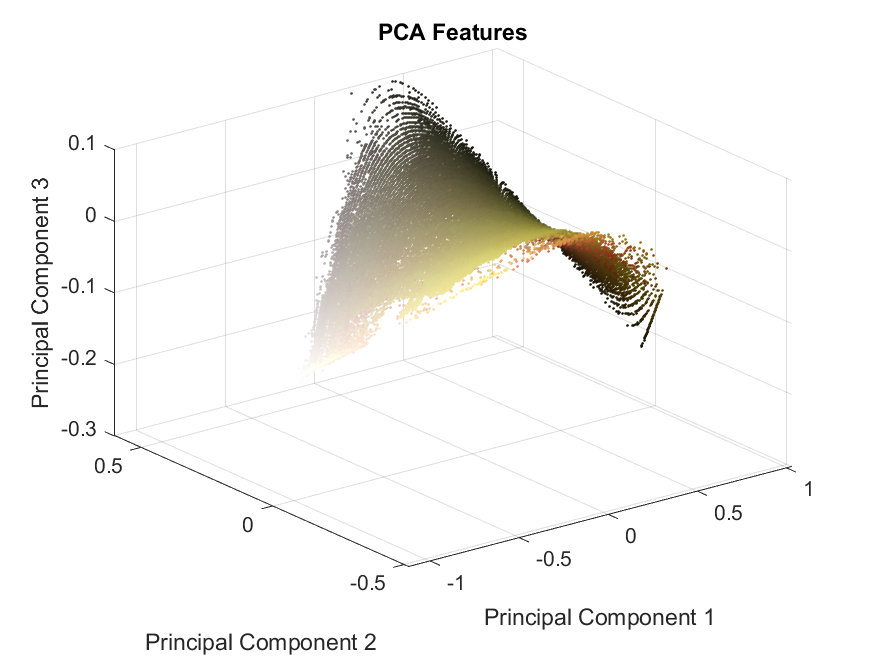
\includegraphics[height=9.5cm, width=\textwidth, keepaspectratio]{Report/Images/Features/Lines/PCAFeatures3D.png}
    \caption{\label{fig:lines:pc 3d}The first 3 principal components}
    \end{figure}
    
    \begin{figure}[H]
    \centering
    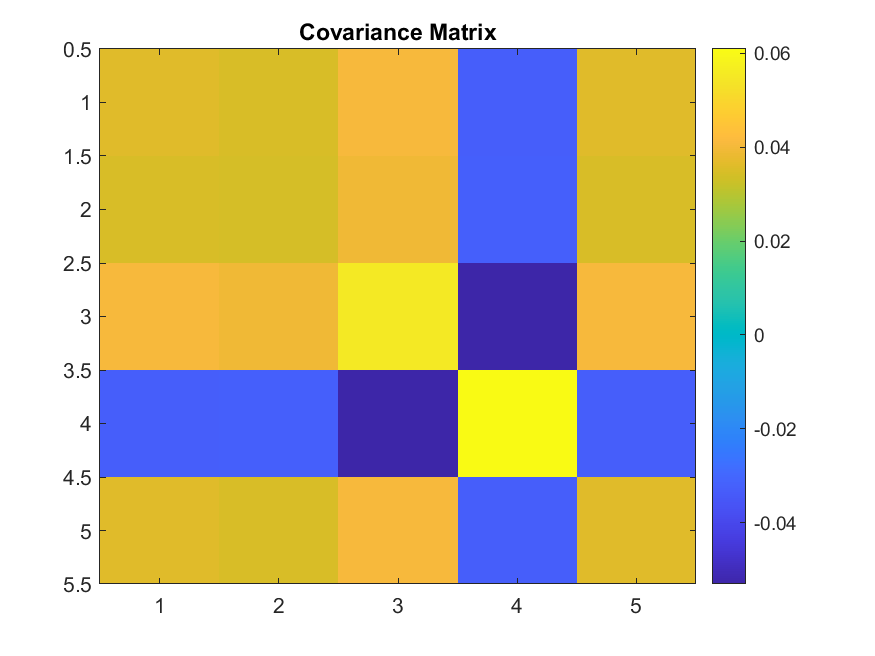
\includegraphics[height=9.5cm, width=\textwidth, keepaspectratio]{Report/Images/Features/Lines/CovarianceMatrix.png}
    \caption{\label{fig:lines:cov}The Covariance matrix between principal components}
    \end{figure}

        \begin{figure}[H]
    \centering
    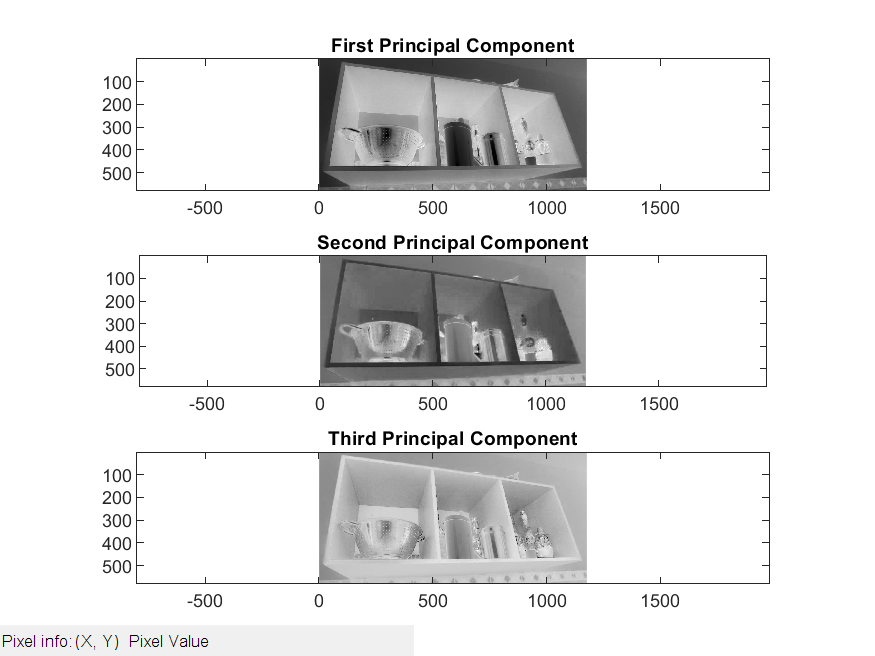
\includegraphics[height=9.5cm, width=\textwidth, keepaspectratio]{Report/Images/Features/Lines/PrincipalComponents.png}
    \caption{\label{fig:lines:cov}The first three principal components in image form}
    \end{figure}

    \item Apply Canny Edge detection to the first principal component

            \begin{figure}[H]
    \centering
    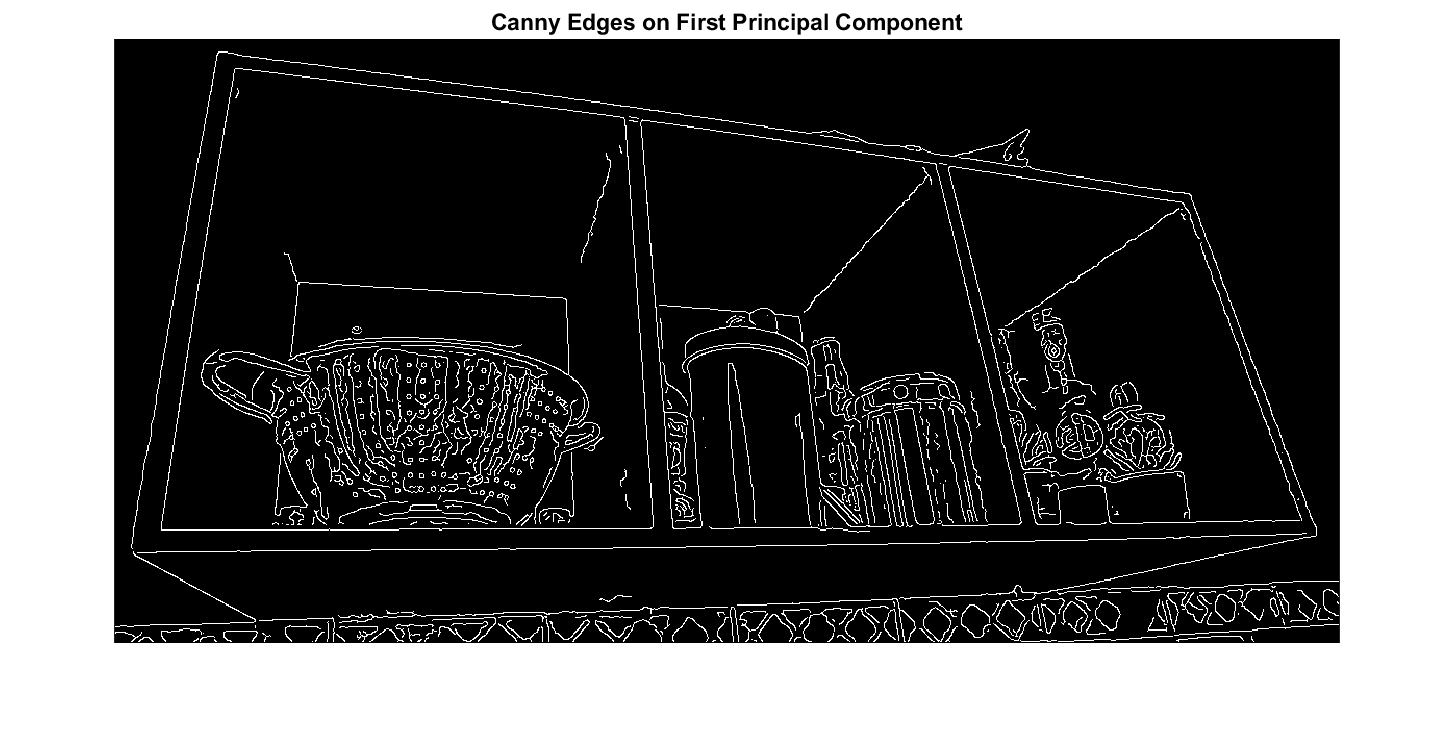
\includegraphics[height=9.5cm, width=\textwidth, keepaspectratio]{Report/Images/Features/Lines/CannyEdges.png}
    \caption{\label{fig:lines:edge}Canny edge detection on the first principal component}
    \end{figure}

    \item Remove edges that are too crowded, like the holes of the colander. To do that, first heavily blur the image then threshold the image to select the sparser areas. Use this to mask the edges.

                \begin{figure}[H]
    \centering
    \includegraphics[height=9.5cm, width=\textwidth, keepaspectratio]{Report/Images/Features/Lines/}
    \caption{\label{fig:lines:edge}Canny edge detection on the first principal component}
    \end{figure}
    
                \begin{figure}[H]
    \centering
    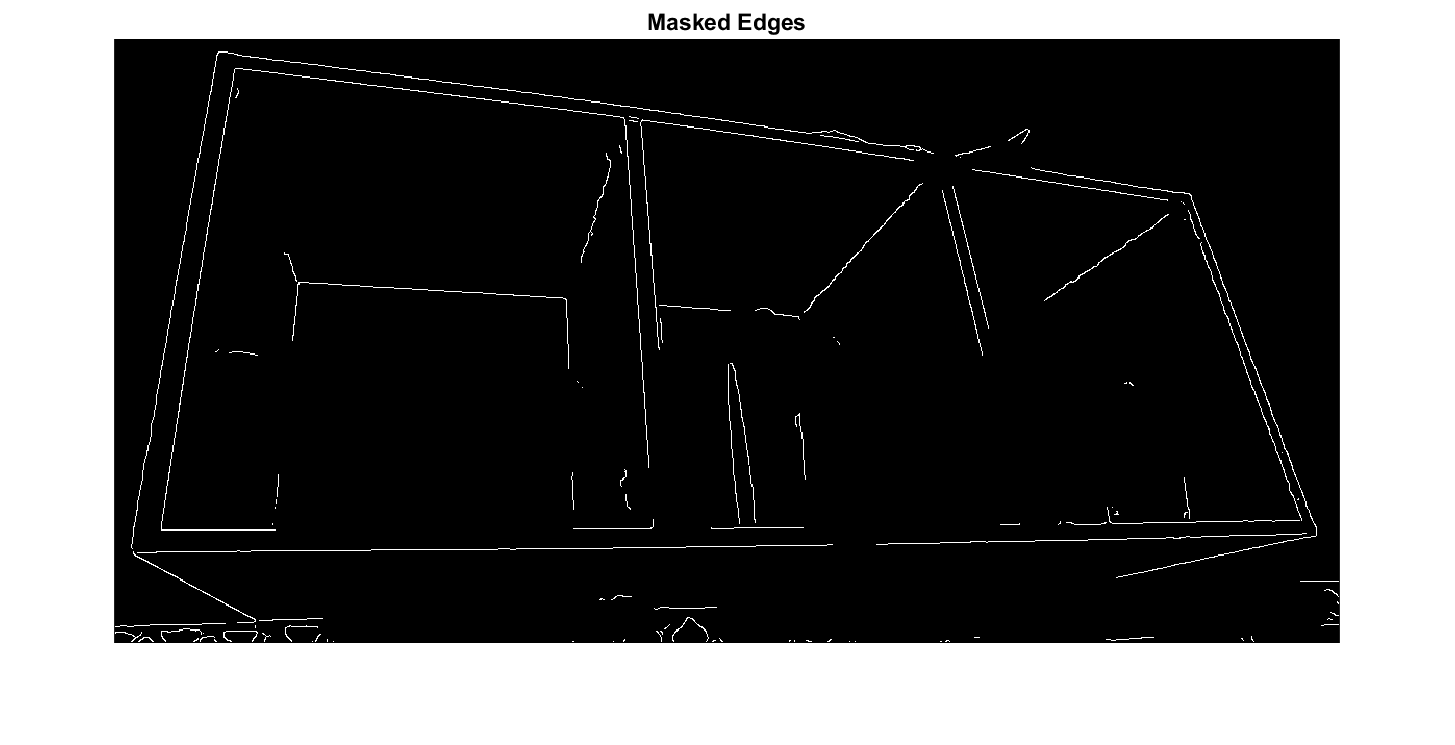
\includegraphics[height=9.5cm, width=\textwidth, keepaspectratio]{Report/Images/Features/Lines/MaskedEdges.png}
    \caption{\label{fig:lines:edge}Canny edge detection on the first principal component}
    \end{figure}

    \item Apply the Hough Transform to the masked edges

                    \begin{figure}[H]
    \centering
    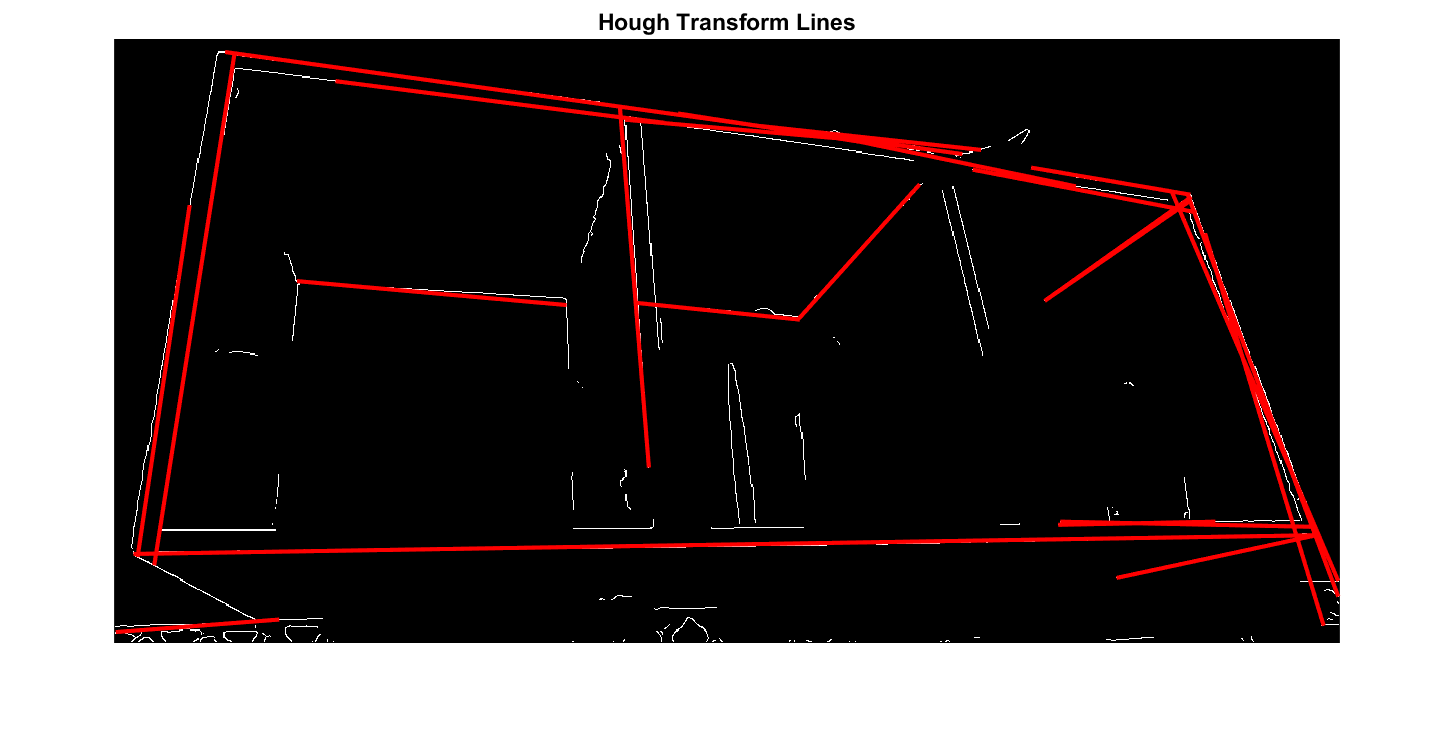
\includegraphics[height=9.5cm, width=\textwidth, keepaspectratio]{Report/Images/Features/Lines/HoughLines.png}
    \caption{\label{fig:lines:lines}Hough Transform result}
    \end{figure}


    
\end{enumerate}

\section{Conic Extraction}
In order to extract the conic $C$:
\begin{enumerate}
    \item Crop the image to the desired portion
    \begin{figure}[H]
    \centering
    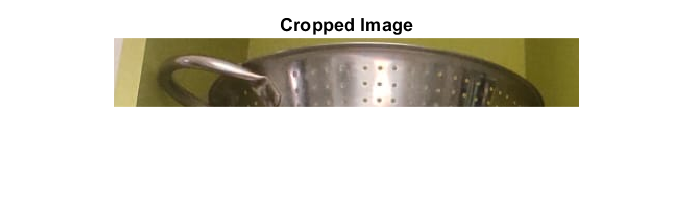
\includegraphics[height=9.5cm, width=\textwidth, keepaspectratio]{Report/Images/Features/Conic/CroppedImage.png}
    \caption{\label{fig:conic:cropped image}The image cropped}
    \end{figure}

    \item Convert to gray scale
    \begin{figure}[H]
    \centering
    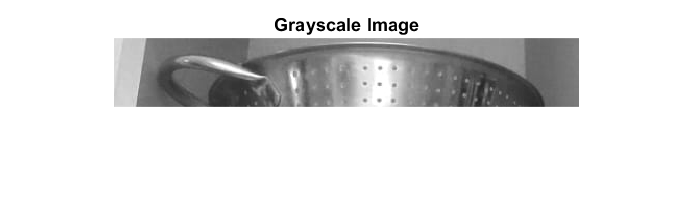
\includegraphics[height=9.5cm, width=\textwidth, keepaspectratio]{Report/Images/Features/Conic/GrayscaleImage.png}
    \caption{\label{fig:conic:gray scale}The image in grey scale}
    \end{figure}

    \item Canny edge detection ($\sigma = 2$, threshold = $[0, 0.15]$)
        \begin{figure}[H]
    \centering
    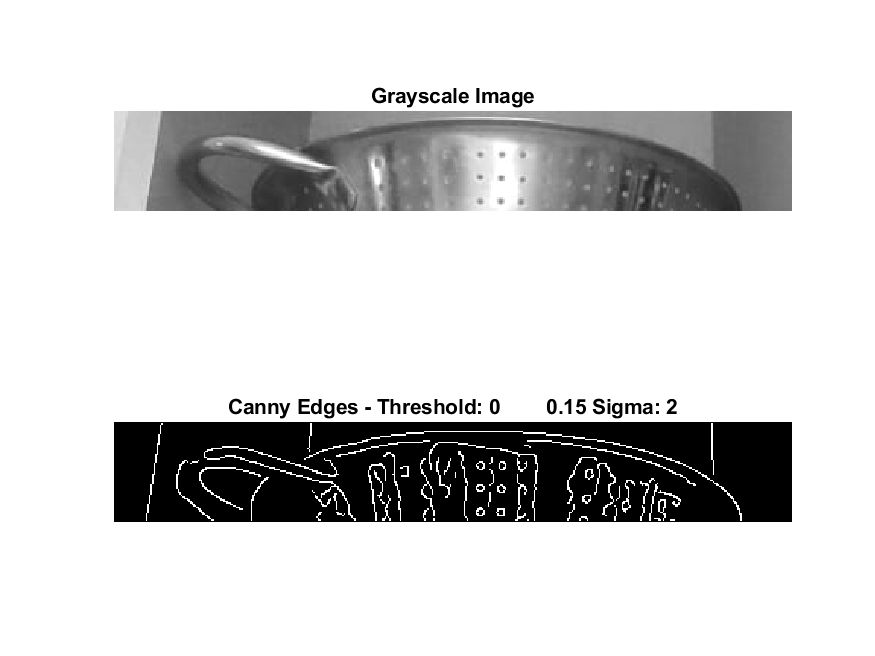
\includegraphics[height=9.5cm, width=\textwidth, keepaspectratio]{Report/Images/Features/Conic/CannyEdges.png}
    \caption{\label{fig:conic:edges}Canny Edge detection}
    \end{figure}

    \item Remove edges that are too crowded, like the holes of the colander. To do that, first heavily blur the image ($\sigma = 10$) then threshold the image to select the sparser areas ($\leq 0.1$). Use this to mask the edges
            \begin{figure}[H]
    \centering
    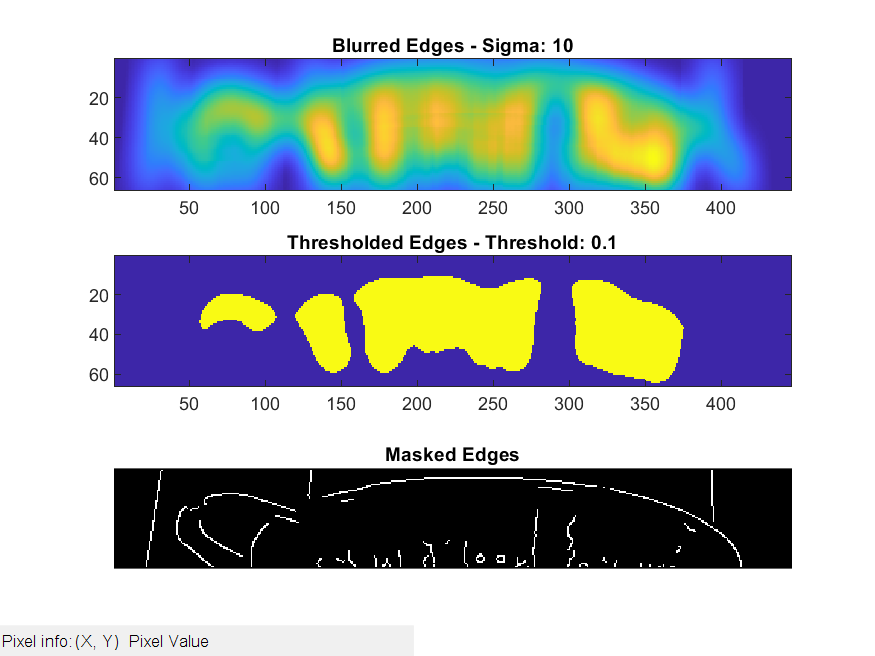
\includegraphics[height=9.5cm, width=\textwidth, keepaspectratio]{Report/Images/Features/Conic/MaskedEdges.png}
    \caption{\label{fig:conic:mask}Masking the edges}
    \end{figure}

    \item Extract the remaining points $\neq 0$ and use a slightly modified RANSAC to extract the Conic with the most inliers 
                \begin{figure}[H]
    \centering
    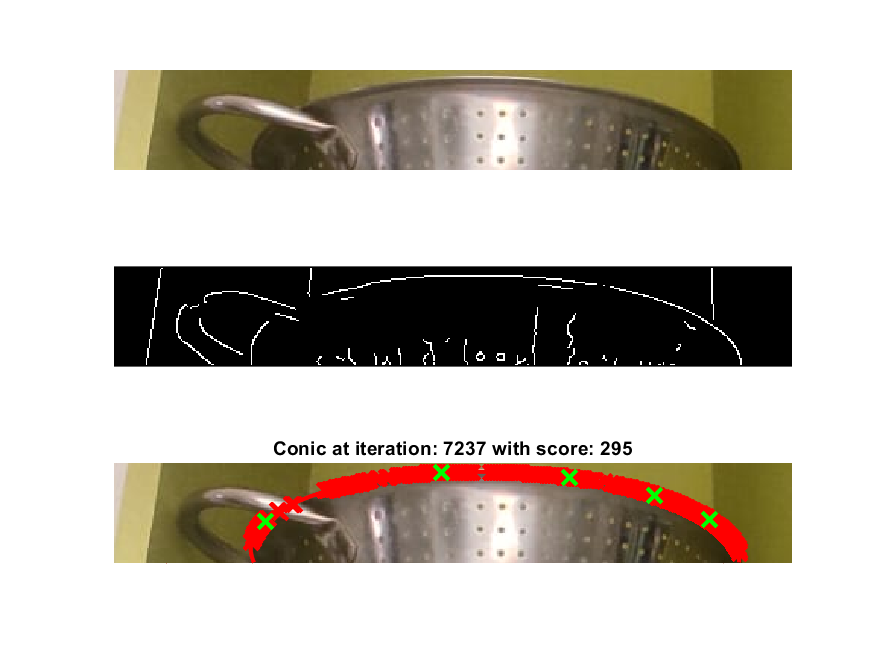
\includegraphics[height=9.5cm, width=\textwidth, keepaspectratio]{Report/Images/Features/Conic/ConicRANSAC.png}
    \caption{\label{fig:conic:ransac}Conic RANSAC}
    \end{figure}

                    \begin{figure}[H]
    \centering
    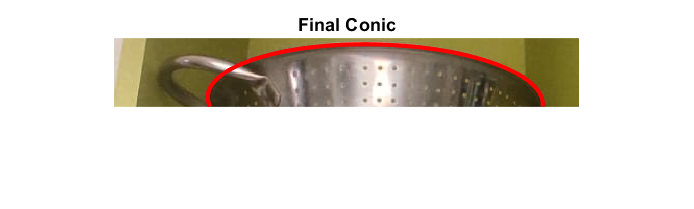
\includegraphics[height=9.5cm, width=\textwidth, keepaspectratio]{Report/Images/Features/Conic/FinalConic.png}
    \caption{\label{fig:conic:final}Final Conic}
    \end{figure}

    
\end{enumerate}

\section{Extraction of $S$ curve}

In order to extract the curve $S$:
\begin{enumerate}
    \item Crop the image to the desired portion
    \item Convert to grayscale
    \item Canny edge detection ($\sigma = 1$, threshold = $[0.2, 0.8]$)
                        \begin{figure}[H]
    \centering
    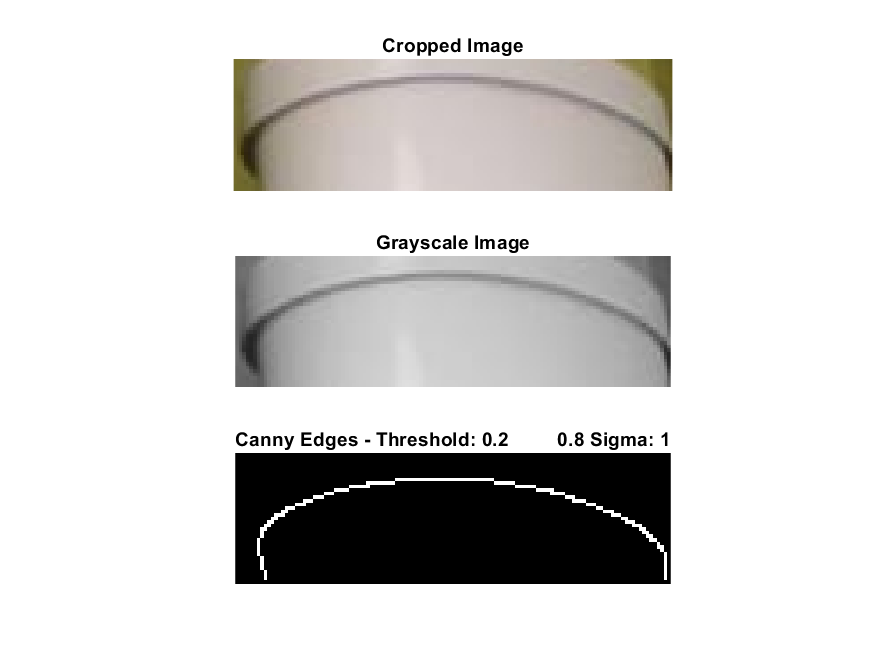
\includegraphics[height=9.5cm, width=\textwidth, keepaspectratio]{Report/Images/Features/S/CannyEdges.png}
    \caption{\label{fig:S extraction}The $S$ extraction process}
    \end{figure}
\end{enumerate}